\documentclass[fr]{../../../../../../eplexam}
\usepackage{tikz}

\hypertitle{Math\'ematique}{3}{FSAB}{1103}{2015}{Août}
{Martin Braquet}
{Jean-François Remacle, Grégoire Winckelmans et Roland Keunings}

\section{Question 2 (25\% des points)}

On considère l'EDP suivante pour $u(x,y)=u(r,\theta)$:
$$\nabla^2 u=\frac{\partial^2 u}{\partial r^2}+\frac{1}{r}\frac{\partial u}{\partial r}+\frac{1}{r^2}\frac{\partial^2 u}{\partial \theta^2}=0$$
et ce à l'intérieur d'un 3/4 de cercle de rayon $a$. Sur l'arc du 3/4 de cercle, on impose que $\frac{\partial u}{\partial n}=\frac{u_0}{a}g(\theta)$, avec $u_0$ un constante de même dimension que $u$ et $g(\theta)$ un fonction adimensionnelle donnée. On impose que $u=0$ sur la face horizontale, et que $\frac{\partial u}{\partial n}=0$ sur la face verticale.
\begin{enumerate}
    \item Faites une esquisse (propre!) du domaine dans le système d'axes physiques $(x,y)$ et une autre dans le système d'axes mathématiques $(r,\theta)$. Indiquez-y clairement les conditions aux limites imposées sur chaque bord, exprimées de façon mathématique.
    \item Utilisez la méthode de séparation des variables pour résoudre le problème. Exprimez la solution sous la forme d'un développement en série (écrire les intégrales à effectuer pour les coefficients du développement!).
\end{enumerate}
\textbf{Rappel}:
$$ rR''+R'=0  \mbox{ a pour solution } R(r)=C\ln r+D$$
$$r^2R''+rR'-k^2R=0 \mbox{ a pour solution } R(r)=Cr^k+Dr^{-k}$$

\begin{solution}

Les esquisses se représentent comme ceci:

\begin{tikzpicture}
      \draw[->] (-2,0) -- (2,0) node[right] {$x$};
      \draw[->] (0,-2) -- (0,1.5) node[above] {$y$};
       \put(-35, 35){$2$}
       \put(20, -10){$1$}
       \put(5, -20){$3$}
      \draw[scale=0.35,domain=0:pi*3/2,smooth,variable=\y,black]  plot ({cos(\y r)*4},{sin(\y r)*4 });
   
      \draw[->] (5,0) -- (7,0) node[right] {$r$};
      \draw[->] (5,0) -- (5,1.5) node[above] {$\theta$};
       \put(160, -10){$1$}
       \put(190, 10){$2$}
       \put(160, 35){$3$}
       \put(130, 10){$4$}
      \draw[-] (5,1) -- (6.5,1);
      \draw[-] (6.5,0) -- (6.5,1);
    \end{tikzpicture}
    
    Les conditions sur les bords sont
\begin{enumerate}
  \item $u(r,0)=0$
  \item $\frac{\partial u}{\partial r}(a,\theta)=\frac{u_0}{a}g(\theta)$
  \item $\frac{\partial u}{\partial \theta}(r,3\pi/2)=0$
  \item partie singulière dans le plan ($r,\theta)$
\end{enumerate}

Par séparation de variable, on écrit u sous la forme
$$ u(r,\theta) = R(r)\Theta(\theta)$$
On l'introduit dans l'EDP et on obtient
$$ \frac{r^2R^{\prime\prime}+rR^{\prime}}{R}=-\frac{\Theta^{\prime\prime}}{\Theta}=\pm k^2 =\lambda$$
On résoud d'abord le mode $\lambda=0$.

La solution pour $\theta$ est 
$$\Theta(\theta)=\overline{A}\theta+B$$
et par la condition 1)
$$\Theta(0)=0 \Rightarrow B=0 \Rightarrow \Theta(\theta)=\overline{A}\theta$$
Mais avec la condition 3),
$$R(r)\Theta'(3\pi/2)= R(r)\overline{A}=0 \Rightarrow \overline{A}=0$$
puisque $R(r)$ ne peut être nulle pour tout $r$ (cela mènerait sinon à la solution nulle pour $u$).

On a donc $\Theta(\theta)=0$ et le mode 0 n'existe pas.

Attaquons nous maintenant au mode $\lambda\neq 0$.

Au vu des conditions homogènes en $\theta$, on choisit $\lambda=+k^2$.

On obtient pour $R(r)$ l'équation
$$r^2R''+rR'-k^2R=0 $$
qui a pour solution
$$R(r)=C\Big(\frac{r}{a}\Big)^k+D\Big(\frac{r}{a}\Big)^{-k}$$
On rentre le $a$ dans l'exposant par facilité par après.

(Note: les aides données à l'examen doivent souvent être utilisées. Il faudrait s'inquiéter si vous n'en avez pas tenu compte dans votre résolution...)

La solution $u$ doit être finie en $(0,0)$, le 2e terme ne convient donc pas. 
$$R(r)=C\Big(\frac{r}{a}\Big)^k$$
On résout pour $\Theta(\theta)$
$$\Theta''+k^2\Theta=0 \Rightarrow \Theta(\theta)=A^*\cos(k\theta) + B^* \sin(k\theta)$$
et 
$$ \Theta(0)=0 \Rightarrow A^*=0\Rightarrow \Theta(\theta)=B^* \sin (k\theta)$$
Par la condition sur le bord 3)
$$\Theta'(3\pi/2)=0\Rightarrow 3\pi k_n/2=(2n-1)\pi/2\Rightarrow k_n=\frac{2n-1}{3}\:(n=1,2,\ldots)$$
Une solution est donc
$$u_{n}(r,\theta)= E_n \sin (k_n\theta)\Big(\frac{r}{a}\Big)^k$$
avec $E_n=B_n^*C$.
Enfin, par le principe de superposition des solutions,
$$u(r,\theta)= \sum\limits_{n=1}^\infty E_n \sin (k_n\theta)\Big(\frac{r}{a}\Big)^k$$
Il reste la dernière condition sur le bord 2) pour déterminer les $E_n$.
$$\frac{\partial u}{\partial r}(r,\theta)=\sum\limits_{n=1}^\infty \frac{E_nk_n}{a} \sin (k_n\theta)\Big(\frac{r}{a}\Big)^{k-1}$$
$$\frac{\partial u}{\partial r}(a,\theta)=\frac{u_0}{a}g(\theta)$$
$$\sum\limits_{n=1}^\infty E_nk_n \sin (k_n\theta)=u_0\:g(\theta)$$
Par othogonalité des fonctions propres
$$\sum\limits_{n=1}^\infty \int^\beta_0\sin(k_n\theta)\sin(k_m\theta)\: d\theta=\int^\beta_0\sin^2(k_m\theta)\:d\theta=\frac{\beta}{2},$$
on a
$$\sum\limits_{n=1}^\infty E_nk_n \int^{3\pi/2}_0 \sin (k_n\theta)\sin(k_m\theta)\:d\theta=\int^{3\pi/2}_0u_0\:g(\theta)\sin(k_m\theta)\:d\theta$$

$$ E_nk_n\frac{3\pi}{4}=u_0\int^{3\pi/2}_0g(\theta)\sin(k_n\theta)\:d\theta$$
La solution est donc
$$u(r,\theta)= \sum\limits_{n=1}^\infty E_n \sin (k_n\theta)\Big(\frac{r}{a}\Big)^k$$
avec 
$$k_n=\frac{2n-1}{3}$$
et
$$ E_n=\frac{4u_0}{3\pi k_n}\int^{3\pi/2}_0g(\theta)\sin(k_n\theta)\:d\theta$$
Il est utile de vérifier les unités, en sachant que les arguments des fonctions (intégrales, exposants) sont adimensionnels, et des sinus sont en radians.

On constate bien que l'intégrale dans $E_n$ est adimensionnelle et que la première fraction a les unités de $u$ ($u_0$) puisque $k_n$ est aussi adimensionnel.

La solution homogène fonctionne tout aussi bien, l'argument du sinus a pour unité des radians, $r/a$ est adimensionnel, et $E_n$ a les unités de $u$.

\begin{solfig}{c}{Solution $u(x,y)$ avec $a=1$ et $g(\theta)=4\sin(10\:\theta)$}
    \centering
    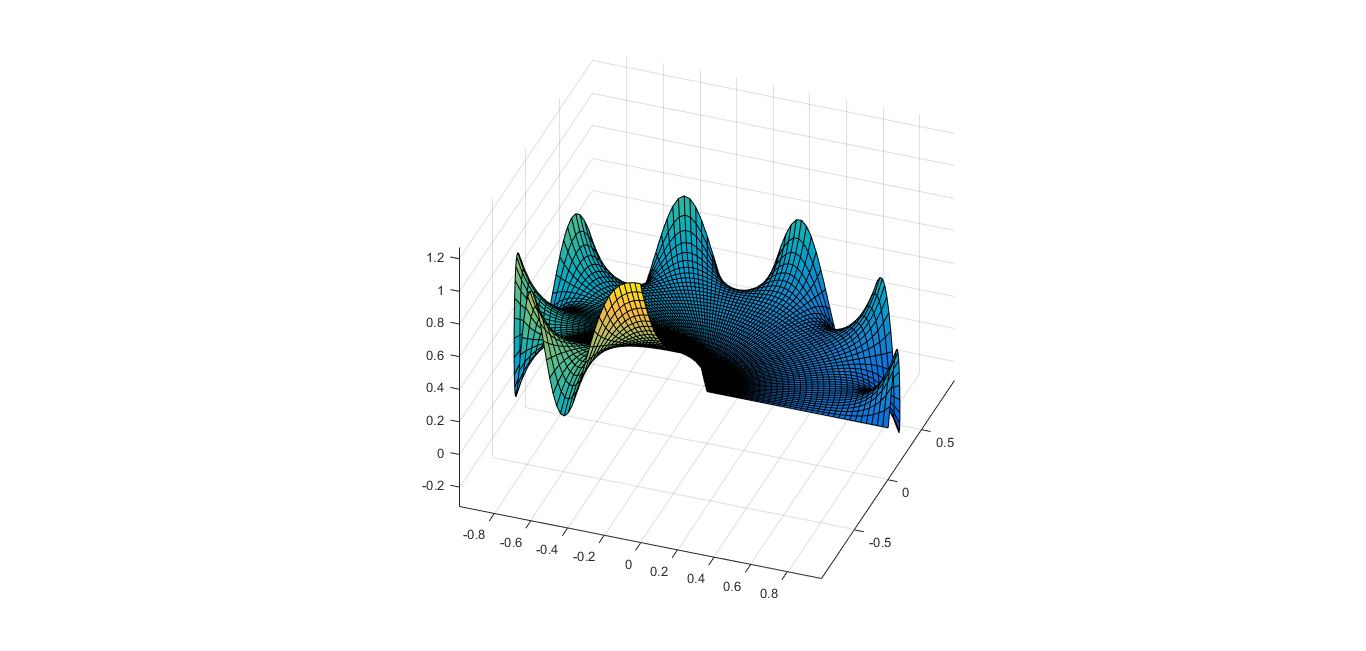
\includegraphics[scale = 0.4]{exam_aout_2015.png}
\end{solfig}

\end{solution}

\end{document}

